% last update november 2019
\documentclass{esannV2}
\usepackage{graphicx}
%\usepackage[latin1]{inputenc}
\usepackage{amssymb,amsmath,array}
\usepackage[utf8]{inputenc}   % Soporte para caracteres UTF-8
\usepackage[spanish]{babel}   % Configuración del idioma español


\usepackage{booktabs}


%***********************************************************************
% !!!! IMPORTANT NOTICE ON TEXT MARGINS !!!!!
%***********************************************************************
%
% Please avoid using DVI2PDF or PS2PDF converters: some undesired
% shifting/scaling may occur when using these programs
% It is strongly recommended to use the DVIPS converters, and to submit
% PS file. You may submit a PDF file if and only if you use ADOBE ACROBAT
% to convert your PS file to PDF.
%
% Check that you have set the paper size to A4 (and NOT to letter) in your
% dvi2ps converter, in Adobe Acrobat if you use it, and in any printer driver
% that you could use.  You also have to disable the 'scale to fit paper' option
% of your printer driver.
%
% In any case, please check carefully that the final size of the top and
% bottom margins is 5.2 cm and of the left and right margins is 4.4 cm.
% It is your responsibility to verify this important requirement.  If these margin requirements and not fulfilled at the end of your file generation process, please use the following commands to correct them.  Otherwise, please do not modify these commands.
%
\voffset 0 cm \hoffset 0 cm \addtolength{\textwidth}{0cm}
\addtolength{\textheight}{0cm}\addtolength{\leftmargin}{0cm}

%***********************************************************************
% !!!! USE OF THE esannV2 LaTeX STYLE FILE !!!!!
%***********************************************************************
%
% Some commands are inserted in the following .tex example file.  Therefore to
% set up your ESANN submission, please use this file and modify it to insert
% your text, rather than staring from a blank .tex file.  In this way, you will
% have the commands inserted in the right place.

\begin{document}
%style file for ESANN manuscripts
\title{Reconocimiento de Actividades Humanas Utilizando Teléfonos Inteligentes}

%***********************************************************************
% AUTHORS INFORMATION AREA
%***********************************************************************
\author{Salgado López Álvaro$^1$
%
% Optional short acknowledgment: remove next line if non-needed
%
% DO NOT MODIFY THE FOLLOWING '\vspace' ARGUMENT
\vspace{.3cm}\\
%
% Addresses and institutions (remove "1- " in case of a single institution)
UANL - Facultad De Ciencias Físico Matemáticas \\
Av. Universidad s/n. Ciudad Universitaria San Nicolás de los Garza - México
}
%
% Remove the next three lines in case of a single institution
%***********************************************************************
% END OF AUTHORS INFORMATION AREA
%***********************************************************************
\maketitle


\section{Introducción}

El Reconocimiento de Actividades Humanas (RAH), constituye un esfuerzo fundamental en el ámbito de comprender el comportamiento humano a través de medios tecnológicos. Su objetivo fundamental radica en identificar las acciones realizadas por individuos basándose en una colección de observaciones derivadas tanto del individuo como de su entorno circundante. Tradicionalmente, las metodologías de reconocimiento han aprovechado diversas fuentes de datos, que van desde señales ambientales hasta sensores colocados en el cuerpo, para lograr este objetivo. Destacadamente, los sensores de movimiento especializados ubicados en varias partes del cuerpo, como la cintura, la muñeca, el pecho y los muslos, han demostrado un rendimiento de clasificación notable. Sin embargo, estas configuraciones de sensores convencionales a menudo conllevan incomodidad para los usuarios y no ofrecen una solución sostenible a largo plazo para el monitoreo de Actividades Humanas (AH).

El advenimiento de los teléfonos inteligentes ha inaugurado una nueva era de oportunidades de investigación en aplicaciones centradas en el ser humano. Con los usuarios como fuentes de información contextual y los teléfonos inteligentes como herramientas de detección primarias, estos dispositivos ubicuos equipados con una variedad de sensores integrados, incluidos acelerómetros, giroscopios, micrófonos y cámaras duales, presentan una alternativa atractiva para el RAH. Al aprovechar los sensores inerciales incorporados en los teléfonos inteligentes, los investigadores han comenzado a explorar vías para monitorear automáticamente y de manera discreta las AH. Notablemente, los teléfonos inteligentes brindan una solución flexible, asequible y autónoma que integra perfectamente el monitoreo de actividades con servicios de telefonía \cite{esann2013}.

En este trabajo, se exploran técnicas de aprendizaje supervisado y no supervisado para clasificar diferentes tipos de HA a partir de datos recogidos por sensores. A diferencia de los métodos supervisados, los algoritmos no supervisados no requieren un conjunto de datos previamente etiquetados para entrenar el modelo, lo cual puede ser ventajoso en escenarios donde la obtención de datos etiquetados es costosa o impráctica.
\section{Marco Teórico}
En el campo de la clasificación de HA mediante datos de sensores, es crucial seleccionar y evaluar adecuadamente los modelos de aprendizaje automático. El RAH tiene aplicaciones en diversos dominios como la salud, el deporte, la seguridad y la interacción humano-computadora. Los datos de sensores, como acelerómetros y giroscopios, proporcionan información importante sobre los movimientos y posturas de una persona, lo que permite identificar diferentes actividades.

\subsection{Métricas de Evaluación}
Para evaluar el rendimiento de los modelos de clasificación, es esencial utilizar métricas adecuadas que proporcionen una visión completa del desempeño del modelo. Las métricas más comunes en el contexto del RAH son:

\subsection*{Exactitud}
La exactitud mide la proporción de predicciones correctas sobre el total de predicciones realizadas.
\begin{equation}
\text{Exactitud} = \frac{\text{Número de predicciones correctas}}{\text{Número total de predicciones}}
\end{equation}

\subsection*{Precisión}
La precisión mide la proporción de verdaderos positivos sobre el total de predicciones positivas.

\begin{equation}
\text{Precisión} = \frac{\text{Verdaderos Positivos}}{\text{Verdaderos Positivos} + \text{Falsos Positivos}}
\end{equation}

\subsection*{Sensibilidad o Tasa de Verdaderos Positivos}
La sensibilidad mide la proporción de verdaderos positivos sobre el total de positivos reales.

\begin{equation}
\text{Sensibilidad} = \frac{\text{Verdaderos Positivos}}{\text{Verdaderos Positivos} + \text{Falsos Negativos}}
\end{equation}

\subsection*{\textit{F1-Score}}
El \textit{F1-Score} es la media armónica de la precisión y la sensibilidad, proporcionando un balance entre ambos.

\begin{equation}
\text{F1-Score} = 2 \times \frac{\text{Precisión} \times \text{Sensibilidad}}{\text{Precisión} + \text{Sensibilidad}}
\end{equation}

\subsection*{Matriz de Confusión}
La matriz de confusión es una tabla que muestra la distribución de predicciones correctas e incorrectas, categorizadas por cada clase. Es una herramienta fundamental para analizar el rendimiento del modelo en cada clase individual.
\subsection{Aprendizaje no supervisado}
Además del popular algoritmo de aprendizaje no supervisado \textit{K-Means}, una alternativa poderosa para abordar el RAH en conjuntos de datos complejos es el Modelo de Mezclas Gaussianas (MMG).

El algoritmo de MMG es especialmente eficaz cuando se trabaja con datos que poseen características continuas, como aquellas obtenidas de sensores de acelerómetro y giroscopio. A diferencia de \textit{K-Means}, que asigna cada punto de datos a un solo agrupamiento, MMG modela la distribución de los datos como una mezcla de varias distribuciones gaussianas. Esto significa que MMG puede capturar la complejidad de conjuntos de datos donde los puntos pueden pertenecer a múltiples grupos.

Un MMG asume que los datos son generados a partir de una combinación (mezcla) de varias distribuciones gaussianas (normales), cada una con su propia media y varianza. Matemáticamente, esto se expresa como:

\begin{eqnarray}
p(x) = \sum_{k=1}^{K} \pi_{k} \mathcal{N}(x | \mu_{k}, \Sigma_{k})
\end{eqnarray}
Donde:

$\mathcal{N}(x | \mu_{k}, \Sigma_{k})$ es una distribución gaussiana con media $\mu_{k}$ y covarianza $\Sigma_{k}$.


$\pi_{k}$ es el peso de la k-ésima componente gaussiana (con $\sum_{k=1}^{K} \pi_{k} = 1$).

%t is your responsibility to verify this important requirement.  If these margin requirements and not fulfilled at the end of your file generation process, please use the commands at the beginning of the ESANNV2.tex file to correct them.  Otherwise, please do not modify these commands.

\subsection{Aprendizaje supervisado}
Se optó por utilizar el algoritmo de Máquinas de Vectores de Soporte (MVS) debido a su eficacia en espacios de alta dimensión, lo cual es ideal para este conjunto de datos ya que contiene características extraídas de múltiples sensores de teléfonos inteligentes, como acelerómetros y giroscopios. Las características en este conjunto de datos pueden ser complejas y altamente dimensionales, y las MVS puede encontrar un hiperplano óptimo que separa eficazmente las diferentes actividades humanas en este espacio de características. Además, algunas variantes de las MSV han demostrado previamente su capacidad en problemas similares, obteniendo buenos resultados \cite{anguitaSVM}.

Las MSV utilizan una función de pérdida Hinge para maximizar el margen y minimizar el error de clasificación:
\begin{eqnarray}
\min_{\mathbf{w}, b} \frac{1}{2} \| \mathbf{w} \|^2 + C \sum_{i=1}^n \max(0, 1 - y_i (\mathbf{w} \cdot \mathbf{x}_i + b))
\end{eqnarray}
Donde:

 \( \| \mathbf{w} \|^2 \) es la norma cuadrada del vector de pesos \( \mathbf{w} \), \( C \) es el parámetro de regularización que controla el \textit{trade-off} entre el margen y el error de clasificación, \( \mathbf{x}_i \) son las muestras de entrenamiento, y \( y_i \) son las etiquetas de clase correspondientes (\( y_i \in \{-1, 1\} \)).

Una vez elegidos los algoritmos para el estudio, el objetivo principal es comparar la eficacia de dos enfoques de aprendizaje automático en la clasificación de actividades humanas: MVS y MMG. El propósito es evaluar y contrastar el rendimiento de estos algoritmos en términos de precisión y capacidad de clasificación.


\section{Metodología}
Se llevaron a cabo una serie de experimentos para obtener el conjunto de datos para el RAH. Se seleccionó un grupo de 30 voluntarios con edades comprendidas entre los 19 y 48 años para esta tarea. A cada persona se le indicó seguir un protocolo de actividades mientras llevaba un teléfono inteligente Samsung Galaxy S II montado en la cintura. Las seis AH seleccionadas fueron estar de pie, sentarse, acostarse, caminar, bajar escaleras y subir escaleras. Cada sujeto realizó el protocolo dos veces: en el primer intento, el teléfono inteligente se colocó en el lado izquierdo del cinturón, y en el segundo, el usuario mismo lo colocó según su preferencia. También hubo una separación de 5 segundos entre cada tarea, donde se les indicaba a los individuos descansar, lo que facilitó la repetibilidad (cada actividad se intentó al menos dos veces) y la generación de datos de referencia a través de la interfaz visual \cite{esann2013}.

\begin{table}[h!]
    \centering
    \resizebox{\textwidth}{!}{%
    \begin{tabular}{|c|l|c|c|l|c|}
        \hline
        \textbf{No.} & \textbf{Estático} & \textbf{Tiempo (seg)} & \textbf{No.} & \textbf{Dinámico} & \textbf{Tiempo (seg)} \\
        \hline
        0 & Inicio (De pie Pos) & 0 & 7 & Caminar (1) & 15 \\
        1 & De pie (1) & 15 & 8 & Caminar (2) & 15 \\
        2 & Sentarse (1) & 15 & 9 & Bajar escaleras (1) & 12 \\
        3 & De pie (2) & 15 & 10 & Subir escaleras (2) & 12 \\
        4 & Acostarse (1) & 15 & 11 & Bajar escaleras (1) & 12 \\
        5 & Sentarse (2) & 15 & 12 & Subir escaleras (2) & 12 \\
        6 & Acostarse (2) & 15 & 13 & Bajar escaleras (3) & 12 \\

        & & & 14 & Subir escaleras (3) & 12 \\
        & & & 15 & Detenerse & 0 \\
        \hline
        \multicolumn{5}{|r|}{\textbf{Total}} & \textbf{192} \\
        \hline
    \end{tabular}
    }
    \caption{Protocolo de actividades para el Experimento RAH.}
    \label{tab:har_protocol}
\end{table}

Las tareas se realizaron en condiciones de laboratorio, pero se les pidió a los voluntarios que realizaran libremente la secuencia de actividades para obtener un conjunto de datos más naturalista. El Cuadro \ref{tab:har_protocol} muestra los detalles del protocolo experimental \cite{esann2013}.


\subsection{Preparación del conjunto de datos}

Al cargar el conjunto de datos, se realizó un mapeo de las etiquetas de las actividades para traducirlas al español, asegurando una interpretación más accesible de los resultados. Además, se llevó a cabo una normalización de los datos para estandarizar las características y garantizar que todas las variables estén en la misma escala, lo cual es crucial para el desempeño de los algoritmos de clasificación.

\subsection{Evaluación del Algoritmo MVS (Aprendizaje Supervisado)}

Para la evaluación del algoritmo MVS, se experimentó con varias configuraciones de parámetros para optimizar su rendimiento. Se probaron diferentes tipos de \textit{kernels}: \texttt{linear}, \texttt{poly} y \texttt{rbf}. Además, se ajustaron los hiperparámetros del modelo, específicamente el parámetro de regularización $C$ (con valores de 0.1, 1 y 10) y el parámetro $\gamma$ (con valores de 0.1, 1 y 10).

Para cada combinación de \textit{kernel} y parámetros, se entrenó el modelo MVS utilizando el conjunto de entrenamiento. Posteriormente, se evaluó el modelo en el conjunto de prueba empleando diversas métricas de desempeño, incluyendo precisión, exactitud, sensibilidad y \textit{F1-Score}. También se calculó la matriz de confusión para examinar detalladamente la distribución de las predicciones correctas e incorrectas, proporcionando una visión completa del rendimiento del modelo.

\subsection{Evaluación del Algoritmo MMG (Aprendizaje No Supervisado)}
Para la evaluación del algoritmo MMG, se exploraron diversas configuraciones de parámetros para determinar el mejor ajuste del modelo. Se experimentó con distintos números de componentes, específicamente 5, 6, y 7, para capturar la complejidad de los datos. Además, se probaron varios tipos de covarianza: \texttt{full}, \texttt{tied}, \texttt{diag} y \texttt{spherical}, cada uno proporcionando una forma distinta de modelar la dispersión de los datos.

Para cada combinación de número de componentes y tipo de covarianza, se ajustó el modelo MMG utilizando el conjunto de entrenamiento. Posteriormente, se calculó la matriz de confusión para analizar cómo se comparan las asignaciones de las agrupaciones con las etiquetas reales, permitiendo una evaluación más completa de la capacidad de clasificación del modelo.


\section{Resultados}
\subsection{Aprendizaje no supervisado}
Luego de implementar el algoritmo de MMG se obtuvo una clasificación de las actividades realizadas.
\begin{figure}[ht!]
\centering
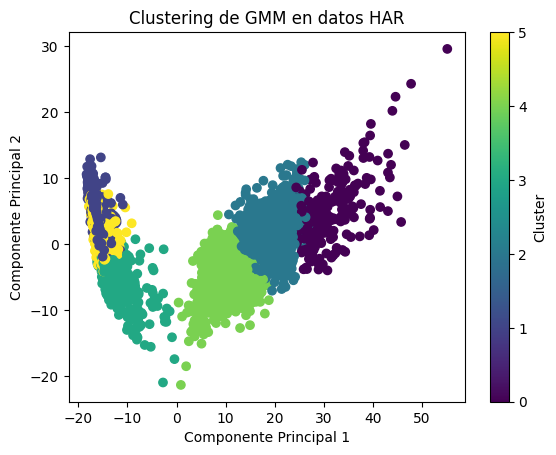
\includegraphics[width=0.5\textwidth]{figs/Resultados.png}
\caption{Agrupamiento de MMG para el RAH}\label{Fig:resultados_MMG}
\end{figure}
Se empleó el algoritmo de MMG para abordar la clasificación de las AH. La Figura \ref{Fig:resultados_MMG} se presenta un análisis de componentes principales, una técnica utilizada para reducir la dimensionalidad de datos complejos. Se observa que varios puntos en el gráfico están superpuestos, lo cual añade dificultad al intentar agrupar los datos utilizando únicamente 2 componentes principales.

\begin{figure}[ht!]
\centering
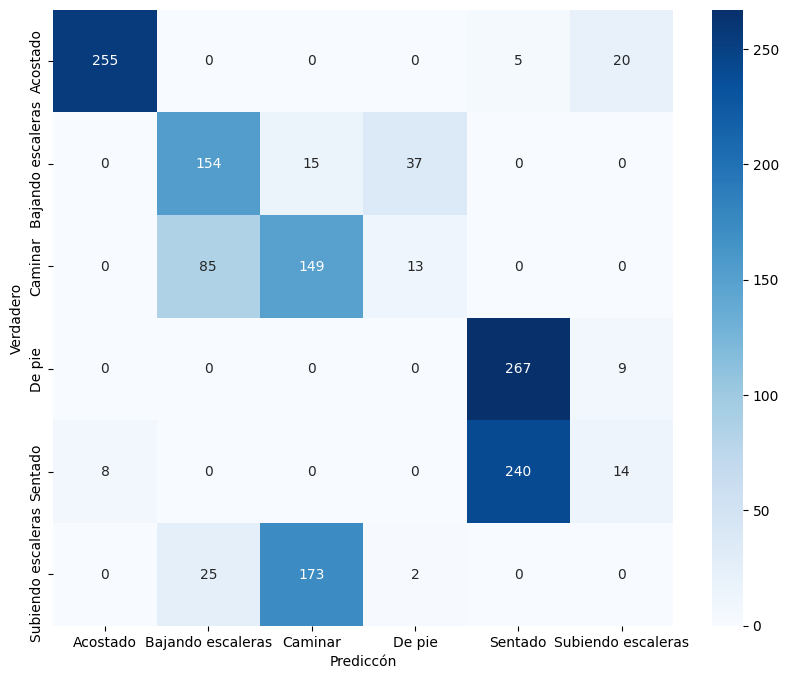
\includegraphics[width=0.5\textwidth]{figs/GMM_matriz.png}
\caption{Matriz de Confusión MMG}\label{Fig:ggm_matriz}
\end{figure}

En la Figura \ref{Fig:ggm_matriz} se observa que el modelo MMG enfrenta dificultades en la clasificación de la actividad de estar de pie, dado que no logró clasificar ningún registro asociado con esta actividad. Este resultado sugiere que el modelo puede no estar capturando adecuadamente las características distintivas o los patrones asociados con la actividad de estar de pie en los datos recopilados. Además, es importante destacar que la exactitud del modelo fue considerablemente baja, alcanzando tan solo un 54\% tal y como se muestra en el Cuadro \ref{tab:classification_report_GGM}. 
\begin{table}[h]
    \centering
    \begin{tabular}{|c|c|c|c|c|}
        \hline
        \textbf{Clase} & \textbf{Precisión} & \textbf{Sensibilidad} & \textbf{F1-Score} & \textbf{Soporte} \\ \hline
        Acostado & 0.97 & 0.91 & 0.94 & 280 \\ \hline
        Bajando escaleras & 0.58 & 0.75 & 0.66 & 206 \\ \hline
        Caminar & 0.44 & 0.60 & 0.51 & 247 \\ \hline
        De Pie & 0.00 & 0.00 & 0.00 & 276 \\ \hline
        Sentado & 0.47 & 0.92 & 0.61 & 262 \\ \hline
        Subiendo escaleras & 0.00 & 0.00 & 0.00 & 200 \\ \hline
        \multicolumn{4}{|c|}{Exactitud} & 0.54 \\ \hline
        \multicolumn{1}{|c|}{Macro Avg} & 0.41 & 0.53 & 0.45 & 1471 \\ \hline
        \multicolumn{1}{|c|}{Weighted Avg} & 0.42 & 0.54 & 0.47 & 1471 \\ \hline
    \end{tabular}
    \caption{Reporte de Clasificación del Algoritmo MMG}
    \label{tab:classification_report_GGM}
\end{table}

Los hallazgos revelan una clasificación deficiente, evidenciada por métricas muy bajas en general. Sería necesario reconsiderar el enfoque actual; posiblemente otros algoritmos podrían ofrecer mejores resultados para mejorar la precisión y efectividad en la clasificación.


\subsection{Aprendizaje Supervisado}
Tras la implementación del algoritmo MVS, se logró alcanzar una precisión del 99\%. Este resultado refleja que el modelo pudo clasificar correctamente un alto porcentaje de los datos del conjunto de prueba, demostrando su eficacia en la tarea de reconocimiento de actividades humanas basadas en datos de sensores de teléfonos inteligentes. La alta precisión obtenida demuestra la capacidad del algoritmo de MVS para manejar de manera efectiva las características complejas y multidimensionales extraídas de los sensores, como acelerómetros y giroscopios.
\begin{figure}[ht!]
\centering
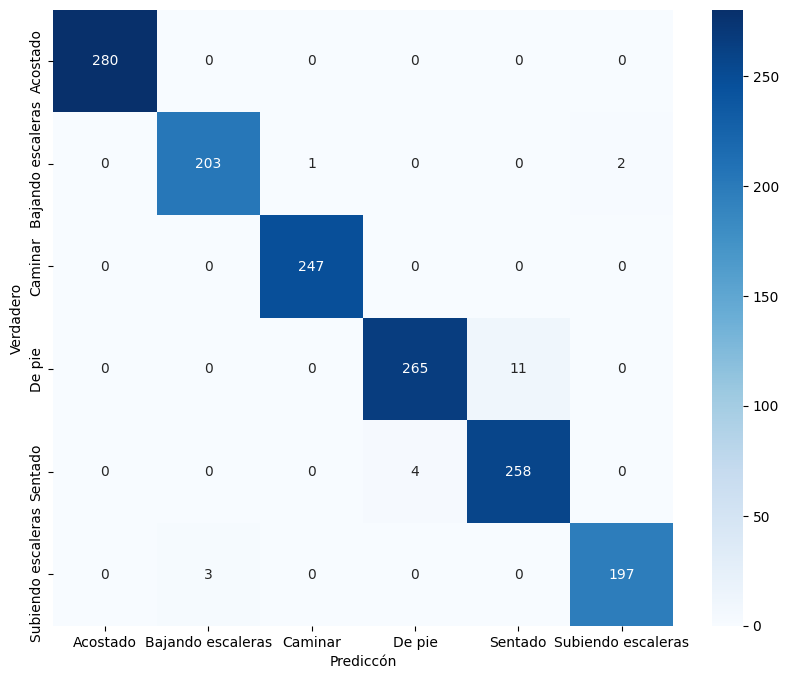
\includegraphics[width=0.5\textwidth]{figs/SVM_matriz.png}
\caption{Matriz de Confusión MVS}\label{Fig:matriz_SVG}
\end{figure}
Además, la Figura \ref{Fig:matriz_SVG} presenta detalladamente la matriz de confusión generada por el modelo. Esta matriz proporciona de manera visual cómo se clasificaron las diferentes actividades, mostrando el número de predicciones correctas e incorrectas para cada clase. Por ejemplo, se observa que la mayoría de las actividades fueron clasificadas con precisión casi perfecta.

El reporte de clasificación presentado en el Cuadro \ref{tab:classification_report} también destaca la sensibilidad (\textit{recall}) del modelo de 99\%, que indica la capacidad del SVM para identificar correctamente las muestras de cada clase. En general, el modelo mostró una alta sensibilidad en todas las actividades, lo que refuerza su robustez y confiabilidad en aplicaciones prácticas.

En la literatura, los resultados del análisis se reportan típicamente en términos de precisión de clasificación utilizando varias métricas estándar como precisión, sensibilidad y \textit{F1-Score}. En general, los estudios investigados reportan una precisión de clasificación muy alta, típicamente superior al 95\%. Por lo tanto, en el Cuadro \ref{tab:classification_report} se presenta el reporte de clasificación obtenido, el cual proporciona una visión detallada del rendimiento del modelo para cada una de las clases en el problema de clasificación de actividades humanas.

\begin{table}[h]
    \centering
    \begin{tabular}{|c|c|c|c|c|}
        \hline
        \textbf{Clase} & \textbf{Precisión} & \textbf{Sensibilidad} & \textbf{F1-Score} & \textbf{Soporte} \\ \hline
        Acostado & 1.00 & 1.00 & 1.00 & 280 \\ \hline
        Bajando escaleras & 0.99 & 0.99 & 0.99 & 206 \\ \hline
        Caminar & 1.00 & 1.00 & 0.99 & 247 \\ \hline
        De pie & 0.99 & 0.96 & 0.97 & 276 \\ \hline
        Sentado & 0.96 & 0.98 & 0.97 & 262 \\ \hline
        Subiendo escaleras & 0.99 & 0.98 & 0.99 & 200 \\ \hline
        \multicolumn{4}{|c|}{Exactitud} & 0.99 \\ \hline
        \multicolumn{1}{|c|}{Macro Avg} & 0.99 & 0.99 & 0.99 & 1471 \\ \hline
        \multicolumn{1}{|c|}{Weighted Avg} & 0.99 & 0.99 & 0.99 & 1471 \\ \hline
    \end{tabular}
    \caption{Reporte de Clasificación del Algoritmo SVM}
    \label{tab:classification_report}
\end{table}

El modelo demostró un rendimiento sobresaliente, con valores de precisión, \textit{recall} y \textit{F1-Score} consistentemente altos en todas las clases. Estos resultados indican que el modelo es altamente eficaz para la clasificación de actividades humanas, lo que lo hace idóneo para aplicaciones en entornos reales donde se requiere una identificación precisa y fiable de las actividades.

\section{Conclusión}
En este estudio, se comparó el desempeño de dos algoritmos de clasificación, uno supervisado MVS y uno no supervisado MMG, para la tarea de clasificación de AH utilizando datos de sensores de teléfonos inteligentes. Los resultados de las métricas de evaluación, incluyendo precisión, sensibilidad, \textit{F1-Score} y la matriz de confusión, mostraron que el modelo de MVS superó consistentemente al modelo MMG en todas las métricas consideradas.

El modelo MVS obtuvo una precisión de clasificación muy alta, con valores de \textbf{F1-Score} superiores al 95\% en todas las clases. Por otro lado, el modelo MMG, aunque logró resultados razonables, no alcanzó el mismo nivel de precisión y consistencia que el de MVS. Estos resultados sugieren que, para el problema específico de clasificación de AH con el conjunto de datos utilizado, el enfoque supervisado del MVS es más eficaz que el enfoque no supervisado del MMG.

Por lo tanto, el MVS se presenta como una solución eficaz y confiable para el reconocimiento de actividades humanas, ofreciendo un alto nivel de precisión y capacidad para gestionar múltiples clases de actividades de manera efectiva. Estos resultados son prometedores para su implementación en sistemas de seguimiento y análisis de actividades diarias, proporcionando una solución robusta y precisa para el monitoreo basado en datos de sensores.


% ****************************************************************************
% BIBLIOGRAPHY AREA
% ****************************************************************************

\begin{footnotesize}

% IF YOU DO NOT USE BIBTEX, USE THE FOLLOWING SAMPLE SCHEME FOR THE REFERENCES
% ----------------------------------------------------------------------------

\bibliographystyle{IEEEtran}
\bibliography{referencias}



% ----------------------------------------------------------------------------

% IF YOU USE BIBTEX,
% - DELETE THE TEXT BETWEEN THE TWO ABOVE DASHED LINES
% - UNCOMMENT THE NEXT TWO LINES AND REPLACE 'Name_Of_Your_BibFile'

%\bibliographystyle{unsrt}
%\bibliography{Name_Of_Your_BibFile}

\end{footnotesize}

% ****************************************************************************
% END OF BIBLIOGRAPHY AREA
% ****************************************************************************

\end{document}
